\chapter{Asynchrone Erweiterungen}
\section{Überblick der Implementierung}
\subsection{Push-Funktionalität zwischen Webserver und --client}
\paragraph{Implementierung mithilfe von STOMP--over--WebSocket}
Zur Realisierung der Websocket Funktionalitäten haben wir die \texttt{Sock.js} und \texttt{Stomp.js} JavaScript Libraries in unser Projekt eingebunden. Zusätzlich mussten wir noch Dependencies in Maven anpassen, sodass die entsprechenden Klassen benutzt werden können.
\begin{verbatim}
<dependency>
    <groupId>org.springframework.boot</groupId>k
    <artifactId>spring-boot-starter-websocket</artifactId>
</dependency>
<dependency>
    <groupId>org.springframework</groupId>
    <artifactId>spring-messaging</artifactId>
</dependency>
\end{verbatim}

Auf jeder Seite, die Benachrichtigungen über neue Posts anzeigen soll, wurde dann über Javascript eine Socket Verbindung aufgebaut (mittels der \texttt{connect()}--Methode aus dem Beispiel) und somit wurde dann der \texttt{Subscribe}--Mechanismus implementiert.\\
Der \texttt{Publish}--Mechanismus wurde in der HTML Seite, die zum Posten von neuen Nachrichten erstellt wurde, implementiert. Hier wird ein \texttt{JSON-Objekt} vor dem Abschicken an den Server per \texttt{AJAX} geschickt. \\ Dieser Request wird von einem speziellen Controller verarbeitet und hierüber dann die abonnierenden Clients informiert. \\
Dieser Controller wird mit den folgenden \texttt{Annotations} versehen:

\begin{verbatim}
@MessageMapping("/hello")
@SendTo("/topic/greetings")
\end{verbatim}

\newpage
\paragraph{Darstellung neuer Nachrichten}
Die Darstellung erfolgt über eine \texttt{Notification}, die anzeigt, wie viele neue Posts seit dem Aktualisieren eingegangen sind. \\
Hierbei wird bei jeder ankommenden Nachricht festgestellt, wie viele Nachrichten bisher eingangen ist und die Anzahl wird erhöht.

\begin{figure}[!htb]
  \begin{center}
      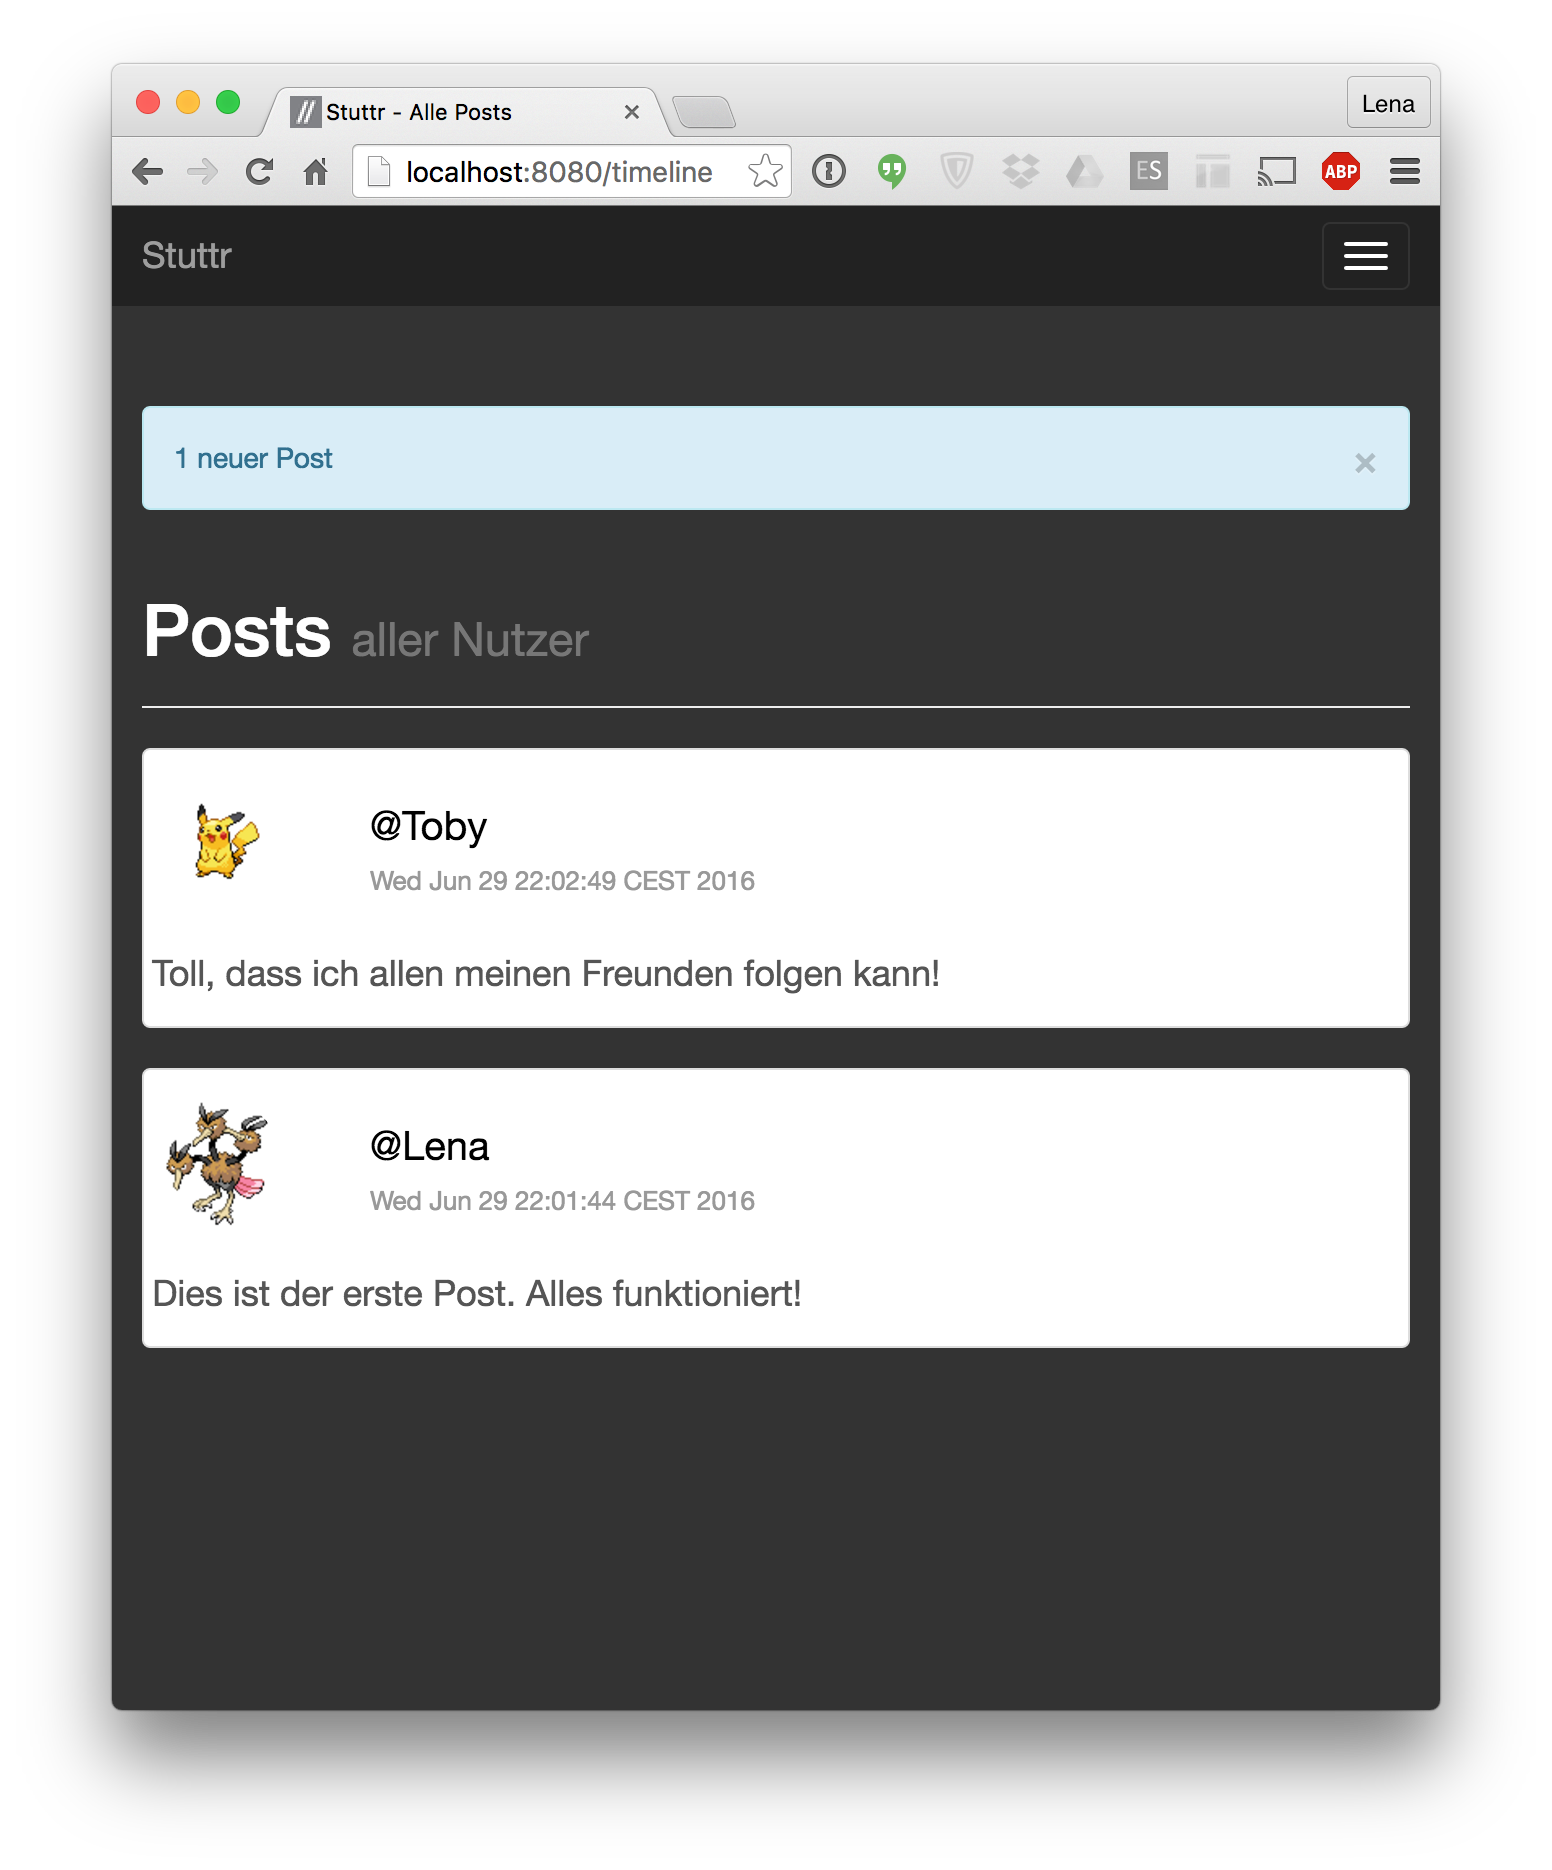
\includegraphics[width=0.75\linewidth]{push}
    \caption{Notification beim Empfangen eines neuen Posts}
    \label{fig:push}
  \end{center}
\end{figure}

Beim Logout wird die Websocket-Verbindung getrennt und somit können keine weiteren Nachrichten empfangen werden.

\newpage
\subsection{Austausch von Updatenachrichten zwischen
Serverinstanzen}
\paragraph{Austausch über Redis Publish-Subscribe-Messaging}
Der Redis Publish-Subscribe--Mechanismus implementiert ein Messaging-System, bei dem Publisher Nachrichten
über einen sogenannten \texttt{Channel} senden können. \\
Ein \texttt{Redis Client} kann eine beliebige Anzahl solcher \texttt{Channels} abonnieren, um dort veröffentlichte Messages automatisch zu empfangen. \\
Will ein \texttt{Client} die Nachrichten eines \texttt{Channels}
nicht mehr empfangen, so kann er diesen deabonnieren (\texttt{unsubscribe}). \\
Für die Konfiguration unserer Anwendung, um diesen Mechanismus umzusetzen, werden in Spring, zusätzlich zu den Beans \texttt{RedisTemplate} und \texttt{ConnectionFactory}, die Beans \texttt{ChannelTopic}, \texttt{MessageListener} und \texttt{RedisPublisher} benötigt. \\
Über die Annotation \texttt{@Schedule} kann festgelegt werden, in welchem
Zeitabstand neue Messages vom Publisher veröffentlicht werden.
